%!TEX root = ../thesis.tex

\section{end-to-end学習}

  end-to-end学習とは,\figref{Fig:about_end-to-end}に示すように,システムの入力から出力までの全体の処理を一つのニューラルネットワークで直接学習する機械学習手法である.この手法では,画像や音声などの特徴抽出や前処理の段階を人手で設計する必要がなく,データから直接目標のタスクを学習することができる.

  \vspace{3cm}

  \begin{figure}[h]
    \centering
    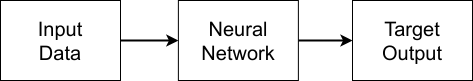
\includegraphics[keepaspectratio, scale=0.70] {images/RobotGuidance_about_end-to-end.png}
    \caption{Structure of end-to-end learning}
    \label{Fig:about_end-to-end}
  \end{figure}

\newpage
